\chapter{微分学基础}\label{chap:calculus}
本书中涉及的积分学很少,并且集中在概率论部分,所以在本附录中我们只讨论微分学,积分学的内容在\Cref{sec:expectation} 中简单介绍. 尽管我们的视角非常一般且抽象,但我们主要讨论的是Euclid空间$\R^n$相关的微分学. 

\section{点集拓扑}\label{sec:topology}
本部分讨论极限、连续、紧致等概念,这些概念是微分学的基础. 

\subsection{度量空间,范数}\label{subsec:metric-norm}
实数集$\R$上面的元素可以被看成一些点,这些点之间有距离的概念. 这是$\R$最重要的几个性质之一. 我们把这种性质抽象出来,得到度量空间的概念. 

\begin{definition}[度量空间]
设$X$是一个集合,$d:X\times X\to\R$是一个函数,如果满足
\begin{enumerate}
    \item 非负性:对任意$x,y\in X$,$d(x,y)\geq 0$,$d(x,y)=0$当且仅当$x=y$;
    \item 对称性:对任意$x,y\in X$,$d(x,y)=d(y,x)$;
    \item 三角不等式:对任意$x,y,z\in X$,$d(x,z)\leq d(x,y)+d(y,z)$. 
\end{enumerate}
则称$(X,d)$是一个\textbf{度量空间},$d$称为\textbf{度量}. 
\end{definition}

下面给出一些度量的例子,但我们不给出验证. 
\begin{example}\label{ex:metric}
    实数集$\R$要成为度量空间,可以装备以下度量:
    \begin{itemize}
            \item 平凡的离散度量:对$x_1\neq x_2$,$d(x_1,x_2)=1$;对$x_1=x_2$,$d(x_1,x_2)=0$. 
            \item 绝对值度量:$d(x_1,x_2)=|x_1-x_2|$. 
        \end{itemize}

        向量空间$\R^n$要成为度量空间,可以装备以下度量:
        \begin{itemize}
            \item Minkowski度量($L^p$度量):$d(x_1,x_2)=(\sum_{i=1}^n|x_1^i-x_2^i|^p)^{1/p}\ (p\geq 1)$. 
            \item Manhattan度量($L^1$度量): $d(x_1,x_2)=\sum_{i=1}^n|x_1^i-x_2^i|$. 
            \item Euclid度量($L^2$度量):$d(x_1,x_2)=\sqrt{\sum_{i=1}^n|x_1^i-x_2^i|^2}$. 
            \item Chebyshev度量($L^\infty$度量): $d(x_1,x_2)=\max_i|x_1^i-x_2^i|=\lim_{p\to\infty}(\sum_{i=1}^n|x_1^i-x_2^i|^p)^{1/p}$. 
        \end{itemize}

    再看一个抽象的例子. 假设$(X,d_X)$和$(Y,d_Y)$是两个度量空间,我们可以定义$X\times Y$上的度量$d$为
    \[d((x_1,y_1),(x_2,y_2))=d_{\R^2}(0,(d_X(x_1,x_2),d_Y(y_1,y_2))).\]
    其中$d_{\R^2}$为$\R^2$上的某个度量. 容易验证这也是一个度量. 
\end{example}

上面关于$\R^n$的例子都有一个特点,他们都是用向量$x_1-x_2$的某种长度定义的,这种长度的概念在数学中有一个统一的抽象,即\textit{范数}. 

\begin{definition}[范数,赋范空间]
设$X$是一个向量空间,$\norm{\cdot}:X\to\R$是一个函数,如果满足
\begin{enumerate}
    \item 非负性与非退化:对任意$x\in X$,$\norm{x}\geq 0$,且$\norm{x}=0$当且仅当$x=0$;
    \item 齐次性:对任意$x\in X$,$\lambda\in\R$,$\norm{\lambda x}=|\lambda|\norm{x}$;
    \item 三角不等式:对任意$x,y\in X$,$\norm{x+y}\leq \norm{x}+\norm{y}$. 
\end{enumerate}
则称$\norm{\cdot}$是$X$上的一个\textbf{范数},$(X,\norm{\cdot})$称为一个\textbf{赋范空间}. 
\end{definition}

容易验证,\Cref{ex:metric} 中的度量都自然地导出了一个范数,即$\norm{x}=d(x,0)$. 我们可以沿袭度量的名字称呼这些范数,例如$L^p$范数就是$L^p$度量所诱导的范数. 很多无穷维线性空间都是先有范数才有空间本身的. 例如,$\ell^p$空间就是由$L^p$范数划定的:
\[ \ell^p=\left\{x\in\C^\infty:\norm{x}_p=\left(\sum_{i=1}^\infty|x_i|^p\right)^{1/p}<\infty\right\}. \]
此外,函数空间$C[a,b]$也可以定义范数,例如
\[ \norm{f}_\infty=\sup_{x\in[a,b]}|f(x)|. \]

反之,任何一个范数都可以导出一个度量,即$d(x,y)=\norm{x-y}$. 这一结论可以总结为如下性质:

\begin{theorem}\label{thm:metric-norm}
    设$X$是一个向量空间,$\norm{\cdot}$是$X$上的一个范数,则$d(x,y)=\norm{x-y}$是$X$上的一个度量,称之为\textbf{范数诱导的度量}. 反之,如果$d$是$X$上的一个度量,则$\norm{x}=d(x,0)$是$X$上的一个范数当且仅当对任意$x,y,z\in X$,$\lambda\in\R$,有
    \begin{enumerate}
        \item 平移不变性:$d(x+z,y+z)=d(x,y)$;
        \item 相似性:$d(\lambda x,\lambda y)=|\lambda|d(x,y)$.
    \end{enumerate}
\end{theorem}

尽管都是$\R^n$,但是不同$p$对应的$L^p$范数是不一样的. 他们之间有如下的关系:

\begin{proposition}\label{prop:lp-norm}
    设$1\leq p\leq q\leq \infty$,则对任意$x\in\R^n$,有
    \[\norm{x}_p\geq \norm{x}_q.\]
\end{proposition}

这一命题的证明依赖于H\"older不等式,这里不给出细节了. 

要想对这一不等式有更好的直观,我们可以考虑$n=2$以及$p=1,2,\infty$的极端情形. 如下图所示,我们要从原点到点$x$. 青色的是$\norm{x}_1=|x_1|+|x_2|$,相当于沿着坐标轴走;而粉色的是$\norm{x}_2=\sqrt{x_1^2+x_2^2}$,相当于沿着对角线走,肯定比沿着坐标轴走要快;紫色的是$\norm{x}_\infty=\max\{|x_1|,|x_2|\}$,相当于挑了较长的那条边走,仿佛虫洞一样,走完了就到了,所以甚至比对角线还快. 

\begin{center}
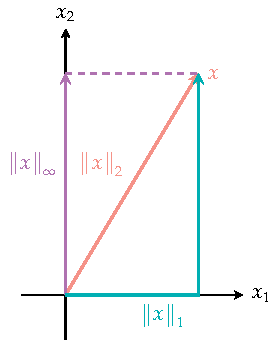
\includegraphics[width=0.45\textwidth]{figures/calculus/norms.pdf}
\end{center}

然而,我们在后面会看到,从拓扑学的角度来说,这些度量并没有本质的区别,这是因为:

\begin{proposition}\label{prop:lp-metric}
    设$1\leq p\leq q\leq \infty$,则存在正常数$c_{p,q}$和$C_{p,q}$,对任意$x,y\in\R^n$,
    \[c_{p,q}\norm{x}_q\leq \norm{x}_p\leq C_{p,q}\norm{x}_q.\]
\end{proposition}

这一证明也依赖于H\"older不等式,所以也略去. 

这一命题说明,虽然不同的范数对应的度量不同,但是他们之间的关系是最多差个常数倍. 我们后面会看到,这一性质表明$L^p$范数定义的所有拓扑性质都是完全相同的. 这一性质也可以一般化:

\begin{definition}[等价范数]
    设$X$是一个向量空间,$\norm{\cdot}_1$和$\norm{\cdot}_2$是$X$上的两个范数,如果存在正常数$c,C$,使得对任意$x\in X$,有
    \[c\norm{x}_1\leq \norm{x}_2\leq C\norm{x}_1,\]
    则称$\norm{\cdot}_1$和$\norm{\cdot}_2$是\textbf{等价}的. 
\end{definition}

\subsection{开集与闭集}

接下来我们进一步进行讨论$\R^n$空间的拓扑性质. 拓扑学是关于开集的学问,给定所有的开集,我们就可以研究一个空间的拓扑性质. 

在$\R$中,很早就已经有了\textit{开区间}的概念,它指的是集合$(a,b)=\{x\in\R:a<x<b\}$. $\R$中的开集定义其实很简单,就是若干开区间的并集. 在更一般的拓扑空间中,开集的定义也是类似的. 我们将视角聚焦在度量空间中. 我们可以把开区间$(a,b)$看成一个圆心在$(a+b)/2$,半径为$(b-a)/2$的一维开球. 从这个视角看,开集的定义是从开球给出的. 这样的定义有一般性:

\begin{definition}[开球,开集,拓扑空间]
    设$(X,d)$是一个度量空间,$x\in X$,$r>0$,定义
    \[B(x,r)=\{y\in X:d(x,y)<r\}.\]
    称$B(x,r)$是以$x$为球心,$r$为半径的\textbf{开球}. 
    
    集合$U\subseteq X$被称为\textbf{开集},如果它是若干开球的并集. 

    $X$连同它的所有开集,被称为\textbf{拓扑空间}\footnote{一般拓扑空间的定义是给出所有开集的集合,并要求他们满足某种封闭性,然而我们这里只关心度量空间,此时可以构造性地给出所有开集. }. 
\end{definition}

在通常的微积分教科书上,我们会看到另一种开集的定义,即开集是任意一点都可以找到一个开球包含在这个集合中. 这两种定义是等价的:

\begin{proposition}\label{prop:open-ball}
    设$(X,d)$是一个度量空间,$U\subseteq X$,则$U$是开集当且仅当对任意$x\in U$,存在$r>0$,使得$B(x,r)\subseteq U$.
\end{proposition}
\begin{proof}
   $\implies$:设$U$是开集,$x\in U$,$U=\bigcup_{i\in I}B(x_i,r_i)$,则存在$i\in I$,使得$x\in B(x_i,r_i)$,取$r=r_i-d(x,x_i)$,显然$r>0$,并且$B(x,r)\subseteq B(x_i,r_i)\subseteq U$.

    $\impliedby$:设对任意$x\in U$,存在$r_x>0$,使得$B(x,r_x)\subseteq U$,则$U=\bigcup_{x\in U}B(x,r_x)$,是开集. 
\end{proof}

本书给的定义是一个更拓扑、更整体的定义:开集就是由基本的开集(开球)经过任意次的并得到的集合,这一定义关心集合而不是具体的点. 而等价的定义,我们称之为\textit{点定义},是更局部的定义,这一定义关心点而不是集合. 今后的定义,我们都尝试用两种方式给出,特别地,拓扑的定义只使用开集而不使用度量. 


我们给几个开集的例子:
\begin{example}[范等价拓扑空间]\label{ex:lp-topology}
    设$X$是一个线性空间,它上面有两个等价的范数$\norm{\cdot}_1$和$\norm{\cdot}_2$\footnote{注意,对一般空间来说,这样的记号不意味着$L^1$或者$L^2$范数. }. 我们要证明,两个赋范空间$(X,\norm{\cdot}_1)$和$(X,\norm{\cdot}_2)$定义了相同的拓扑空间. 因此,在拓扑意义下,$\R^n$空间到底装备了哪个$L^p$范数是不重要的,因此对于同一个数学对象(集合、序列、函数)来说,收敛性和连续性在$L^p$范数下都是完全一样的. 

    下面我们来证明这一点. 我们用开集的点定义. 设$U$是$(X,\norm{\cdot}_1)$中的开集,$x\in U$,则存在$r>0$,使得$B_1(x,r)\subseteq U$,由范数等价,存在$c,C>0$,使得$c\norm{x}_2\leq \norm{x}_1\leq C\norm{x}_2$,则$B_2(x,r/c)\subseteq B_1(x,r)\subseteq U$,所以$U$是$(X,\norm{\cdot}_2)$中的开集. 反之亦然. 
\end{example}

\begin{example}[乘积拓扑空间]\label{ex:product-topology}
    设$(X_1,d_1)$和$(X_2,d_2)$是两个度量空间,则$X_1\times X_2$上的开集有两种自然的方式给出:
    \begin{enumerate}
        \item 对任意开集$U_1\subseteq X_1$和$U_2\subseteq X_2$,定义$U_1\times U_2$是$X_1\times X_2$上的开集,然后利用这些基本的开集的任意并给出所有开集;
        \item 规定$X_1\times X_2$上的度量$d$,然后利用这个度量给出开集. 
    \end{enumerate}

    把度量$d$定义为
    \[d((x_1,y_1),(x_2,y_2))=\norm{(d_1(x_1,x_2),d_2(y_1,y_2))},\]
    其中$\norm{\cdot}$是$\R^2$的某个$L^p$范数. 可以证明,这两种方式给出了$X_1\times X_2$上相同的拓扑. 
    
    因此,以后讨论“拓扑空间$X\times Y$”的地方,不管明里暗里,所指的拓扑空间都是由这两种等价方式给出的. 这一结论可以推广到任意有限个度量空间的乘积. 
\end{example}

开集的重要性质是:

\begin{proposition}\label{prop:open-prop}
    设$(X,d)$是一个非空度量空间,则
    \begin{enumerate}
        \item $X$和$\varnothing$是开集;
        \item 任意个开集的并集是开集;
        \item 有限个开集的交集是开集. 
    \end{enumerate}
\end{proposition}
\begin{proof}
\begin{enumerate}
    \item 取$x\in X$,则$X=\bigcup_{r>0}B(x,r)$,是开集. $\varnothing$是零个(也是若干个)开集的并集,是开集. 

    \item 设$\{U_i\}_{i\in I}$是一族开集,$U_i=\bigcup_{j\in J_i} B(x_j,r_j)$,显然$U=\bigcup_{i\in I}U_i=\bigcup_{i\in I,j\in J_i} B(x_j,r_j)$,是开集. 

    \item 设$U_1,\dots,U_n$是开集,$U=\bigcap_{i=1}^nU_i$,对任意$x\in U$,对任意$i=1,\dots,n$,$x\in U_i$,由开集的点定义,存在$r_i>0$,使得$B(x,r_i)\subseteq U_i$,取$r=\min_{i=1}^n r_i$,则$B(x,r)\subseteq U_i$,所以$U$是开集. 
\end{enumerate}
\end{proof}

注意,开集只对有限交封闭. 可以看一个简单的例子:$\bigcap_{n=1}^\infty(-1/n,1/n)=\{0\}$,但是$\{0\}$不是开集,因为这个集合不可能包含任何开球. 

\Cref{prop:open-prop} 其实就是一般拓扑空间中开集要满足的三条公理. 我们之所以将它写为命题,是因为我们的开集定义基于度量空间,而非一般的拓扑空间.

与开集相对应的是闭集的概念. 闭集的定义是:

\begin{definition}[闭集]
    设$(X,d)$是一个度量空间,$F\subseteq X$,如果$X\setminus F$是开集,则称$F$是\textbf{闭集}. 
\end{definition}
闭集的定义是开集的对偶,所以有如下性质:

\begin{proposition}\label{prop:closed-prop}
    设$(X,d)$是一个非空度量空间,则
    \begin{enumerate}
        \item $X$和$\varnothing$是闭集;
        \item 任意个闭集的交集是闭集;
        \item 有限个闭集的并集是闭集. 
    \end{enumerate}
\end{proposition}

开集和闭集的定义是对偶的,但是性质却完全不同. 开集似乎可以简单理解为开区间的推广,即把开区间拼起来,它的构造是“把东西放进来”. 闭集是把若干开区间挖出来得到的集合,它的构造方式是“把东西拿出去”,这样的构造对我们来说是不够直观的. 我们可以构造非常奇怪的闭集,例如Cantor集就是例子. 

\subsection{紧致性,收敛性,完备性}

接下来我们讨论一个更微妙的概念,\textit{紧致性}或者\textit{紧集}. 紧致性与极限、收敛、连续等概念有着密切的联系,然而如何恰当的定义紧致性是一个很难的问题. 我们这里不讨论历史,只给出历史的答案. 简单来说,\textit{紧}这个词的概念是\textit{压缩},将无穷多的东西变成有限个. 我们的逻辑推理只能处理有限的东西,所以紧致性是沟通无穷和有限的桥梁. 下面给出紧集的定义:

\begin{definition}[开覆盖,紧集]
    设$(X,d)$是一个度量空间,$F\subseteq X$,如果存在一族开集$\{U_i\}_{i\in I}$,使得$F\subseteq \bigcup_{i\in I}U_i$,则称$\{U_i\}_{i\in I}$是$F$的一个\textbf{开覆盖}. 
    
    如果对任意$F$的开覆盖$\{U_i\}_{i\in I}$,都存在有限子覆盖$\{U_{i_j}\}_{j=1}^n$,使得$F\subseteq \bigcup_{j=1}^nU_{i_j}$,则称$F$是\textbf{紧集}. 
\end{definition}

第一次看到这样的定义大概率会不知所云. 然而,我们没有办法将它还原为更直观的定义了. 例如,即便在最基本的集合$\R$上,紧集的存在性也只能被作为与实数公理\footnote{当然,这样的说法把实数集作为一个数学对象,试图用公理定义出来,而不是从已有的数学对象构造出来(例如Dedekind分割). }等价的命题存在:

\begin{proposition}[Heine-Borel有限覆盖原理]\label{prop:heine-borel}
设$F$是$\R$的一个闭区间,对任意$F$开覆盖$\{U_i\}_{i\in I}$,存在有限子覆盖$\{U_{i_j}\}_{j=1}^n$.
\end{proposition}

这一原理说明,闭区间是紧集,因而给出了$\R$中紧集的存在性. 

在度量空间上,紧集与收敛性密切相关. 为此,我们需要形式地定义度量空间中的收敛概念. 我们先使用$\epsilon-N$语言定义:

\begin{definition}[收敛,极限]
    设$(X,d)$是一个度量空间,$\{x_n\}_{n=1}^\infty$是$X$中的一个序列,$x\in X$,如果对任意$\epsilon>0$,存在$N\in\N$,使得对任意$n>N$,$d(x_n,x)<\epsilon$,则称$\{x_n\}_{n=1}^\infty$\textbf{收敛}到$x$,记作$\lim_{n\to\infty}x_n=x$或$x_n\to x$,$n\to\infty$,$x$称为$\{x_n\}_{n=1}^\infty$的\textbf{极限}. 
\end{definition}

这一定义描绘了一幅图像:一列点越来越接近某个点$x$. 如果我们将定义中的$N$取掉,这一直观会更清楚:对任意$\epsilon>0$,除掉有限个$n$(也就是前$N$个),都有$x_n\in B(x,\epsilon)$. 所谓越来越接近,指的就是画任意一个球$B(x,\epsilon)$,除去有限个$x_n$,剩下的所有$x_n$都在这个球里面. 这一想法给出了只基于开集的等价定义:

\begin{proposition}\label{prop:converge-ball}
    设$(X,d)$是一个度量空间,$\{x_n\}_{n=1}^\infty$是$X$中的一个序列,$x\in X$,则$\{x_n\}_{n=1}^\infty$收敛到$x$当且仅当对任意包含$x$的开集$U$,存在$N\in\N$,使得对任意$n>N$,$x_n\in U$.
\end{proposition}
\begin{proof}
    $\implies$:设$\{x_n\}_{n=1}^\infty$收敛到$x$,$U$是包含$x$的开集,由开集的点定义,存在$r>0$,使得$B(x,r)\subseteq U$,由收敛的定义,存在$N\in\N$,使得对任意$n>N$,$d(x_n,x)<r$,所以$x_n\in B(x,r)\subseteq U$.

    $\impliedby$:设对任意包含$x$的开集$U$,存在$N\in\N$,使得对任意$n>N$,$x_n\in U$,则对任意$\epsilon>0$,取$U=B(x,\epsilon)$,则存在$N\in\N$,使得对任意$n>N$,$x_n\in B(x,\epsilon)$,即$d(x_n,x)<\epsilon$,所以$\{x_n\}_{n=1}^\infty$收敛到$x$.
\end{proof}

在一般的拓扑空间中,甚至都没有度量的概念,然而,开集定义收敛依然是可以的. 这正是这一命题的意义. 

下面给一些收敛的经典例子:
\begin{example}
\begin{itemize}
    \item 在$\R$中,$\{1/n\}_{n=1}^\infty$收敛到$0$,然而,序列$\{n\}_{n=1}^\infty$则不收敛. 这个例子表明,极限未必需要在序列中出现,以及趋于无穷是一种特殊的不收敛.
    \item 在$\R^n$和$L^p$范数下,$\{x_k\}_{k=1}^\infty$收敛到$x$,当且仅当对任意$i=1,\dots,n$,$\{x_k^i\}_{k=1}^\infty$收敛到$x^i$,其中$x_k=(x_k^1,\dots,x_k^n)$,$x=(x^1,\dots,x^n)$. 这个例子表明,高维空间中的收敛性可以从每个分量看. 
    \item 在$C([0,1])$和$L^\infty$范数下,$f_n\to f$实际上是所谓\textbf{一致收敛}的概念,即对任意$\epsilon>0$,存在不依赖$x$的$N\in\N$,使得对任意$n>N$,任意$x\in[0,1]$,$|f_n(x)-f(x)|<\epsilon$. 在这一概念下,$\{x^n\}_{n=1}^\infty$就不收敛(尽管它逐点收敛). 
\end{itemize}
\end{example}

度量空间中紧集可以完全由收敛性来刻画:

\begin{theorem}\label{thm:compact-converge}
    设$(X,d)$是一个度量空间,$F\subseteq X$,则$F$是紧集当且仅当$F$中的任意序列都有收敛子列. 
\end{theorem}

这一定理的证明并不算困难,但是需要陈述的事实较多,且与本书关联不大,所以这里都略去. 

\Cref{thm:compact-converge} 足以表明紧集这一概念的重要性了. 然而,这一定理的成立只需要度量空间,度量空间是一个非常弱的概念,我们关心的$\R^n$空间实际上有更强的性质,这一性质是\textit{完备性}. 要定义完备性,我们需要\textit{Cauchy列}. 

\begin{definition}[Cauchy列]
    设$(X,d)$是一个度量空间,$\{x_n\}_{n=1}^\infty$是$X$中的一个序列,如果对任意$\epsilon>0$,存在$N\in\N$,使得对任意$m,n>N$,$d(x_m,x_n)<\epsilon$,则称$\{x_n\}_{n=1}^\infty$是一个\textbf{Cauchy列}. 
\end{definition}

Cauchy列描述了另一种收敛的概念,它要求的是序列中的点越来越相互接近,而不是越来越接近某个点. 注意,这一定义没有办法像收敛性一样给一个纯拓扑的定义,所以Cauchy列的概念是依赖于度量的. 

Cauchy列与收敛列的关系如下. 首先,收敛的点列是Cauchy列:

\begin{proposition}\label{prop:cauchy-converge}
    设$(X,d)$是一个度量空间,$\{x_n\}_{n=1}^\infty$是$X$中的一个序列,如果$\{x_n\}_{n=1}^\infty$收敛,则$\{x_n\}_{n=1}^\infty$是Cauchy列. 
\end{proposition}
\begin{proof}
    设$\{x_n\}_{n=1}^\infty$收敛到$x$,则对任意$\epsilon>0$,存在$N\in\N$,使得对任意$n>N$,$d(x_n,x)<\epsilon/2$,所以对任意$m,n>N$,$d(x_m,x_n)\leq d(x_m,x)+d(x,x_n)<\epsilon$,所以$\{x_n\}_{n=1}^\infty$是Cauchy列. 
\end{proof}

反过来,Cauchy列是否一定收敛呢?这一问题的答案是不一定. 在$\R$上,就如同有限覆盖原理,这件事的成立性只能作为与实数公理等价的命题存在!完备性指的就是Cauchy列一定收敛的性质:

\begin{definition}[完备度量空间]
    设$(X,d)$是一个度量空间,如果$X$中的任意Cauchy列都收敛,则称$(X,d)$是一个\textbf{完备度量空间}. 
\end{definition}
我们不加证明地给出完备度量空间的例子:
\begin{example}
\begin{itemize}
\item 有限维空间的例子:$L^p$范数下$\R^n$是完备的.
\item 反面的例子:使用度量$d(x_1,x_2)=|x_1-x_2|$,则$X=\R\setminus\{0\}$不是完备度量空间. 考虑$\{x_n=\frac1n:n\in\N\}$,它是Cauchy列,但该点列在$X$中没有极限(极限是$0$).
\item 无穷维空间的例子:$[0,1]$到$\R$的连续函数空间$C([0,1])$在$L^\infty$范数下是完备的.
\item 无穷维空间的另一个例子:$\ell^p$空间是完备的. 
\end{itemize}
\end{example}

最后我们指出,尽管完备度量空间已经足够发展微积分了,但是它和$\R^n$依然有一个本质的区别,这一区别在于紧集. 首先,在有限维情况下,紧集与有界闭集是等价的:

\begin{theorem}\label{thm:compact-bounded}
设$\R^n$装备了$L^p$范数,设$F\subseteq\R^n$,那么$F$是紧集当且仅当$F$是有界闭集,有界指的是存在$M>0$,使得对任意$x\in F$,$\norm{x}_p\leq M$.
\end{theorem}

这一命题的证明依赖于Heine-Borel有限覆盖原理,这里就不给出细节了. 

然而,在无穷维空间中,这一命题不一定成立:

\begin{proposition}\label{prop:compact-not-bounded}
设$\ell^2$空间的标准正交向量组是$\{e_i\}_{i=1}^\infty$,$e_i$是第$i$个分量为$1$,其他分量为$0$的向量. 考虑单位球面$E=\{x\in\ell^2:\norm{x}_2=1\}$,则$E$是有界闭集,但不是紧集. 
\end{proposition}
\begin{proof}
    因为对任意$x\in E$,$\norm{x}=1$,所以$\norm{x}_2\leq 1$,所以$E$是有界集. 取$x\in\ell^2\setminus E$. 如果$\norm{x}=r<1$,那么开球$B(x,(1-r)/2)\subseteq B(0,1)\subseteq \ell^2\setminus E$;对于$r>1$可以同理讨论. 这就证明了$E$是闭集. 最后证明$E$不是紧集. 考虑序列$\{e_i\}_{i=1}^\infty$,它是$E$中的序列,因为对任意不同的$m,n$,$\norm{e_m-e_n}=2$,因此$\{e_i\}$的任何子列都不是Cauchy列,根据\Cref{prop:cauchy-converge} 的逆否命题,$\{e_i\}$没有任何收敛子列,因而根据\Cref{thm:compact-converge},$E$不是紧集. 
\end{proof}

\subsection{连续映射}
接下来我们讨论两个拓扑空间之间的映射. 我们说过,拓扑空间完全由开集给出,所以某种程度保持拓扑性质的映射也会与开集有关系. 对于微积分来说,连续性是其中最重要的一种. 遵循先前的惯例,我们先给出更像微积分的$\delta$-$\epsilon$语言的点定义,然后再给出更像拓扑的定义. 

$\delta$-$\epsilon$语言的定义是从\textit{映射的极限}这一概念出发的:

\begin{definition}[映射的极限]
    设$(X,d_X)$和$(Y,d_Y)$是两个度量空间,$f:X\to Y$是一个映射,$x_0\in X$,$y\in Y$,如果对任意$\epsilon>0$,存在$\delta>0$,使得对任意$x\in X$,如果$0<d_X(x,x_0)<\delta$,则$d_Y(f(x),y)<\epsilon$,则称$y$是$f$在$x_0$处的\textbf{极限},记作$\lim_{x\to x_0}f(x)=y$或$f(x)\to y$,$x\to x_0$.
\end{definition}

注意,定义中我们划定了$x$的范围,即$x\neq x_0$. 此时极限的概念由去心邻域$B(x_0,\delta)\setminus\{x_0\}$给出,这样做允许极限并不等于$f(x_0)$本身. 

\begin{remark}
映射的极限还可以定义自变量趋于无穷、单侧极限以及其他情况,我们后面会使用这些概念,他们的直观含义都是明确的,这里我们不再给出正式定义,我们只给出他们的记号:
\begin{itemize}
    \item 趋于无穷:$\lim_{x\to\infty}f(x)=y$或$f(x)\to y$,$x\to\infty$;
    \item 如果定义域是$\R$,还可以定义趋于正、负无穷:$\lim_{x\to+\infty}f(x)=y$或$f(x)\to y$,$x\to+\infty$,$\lim_{x\to-\infty}f(x)=y$或$f(x)\to y$,$x\to-\infty$;
    \item 单调递增趋于:$x\uparrow x_0$,单调递减趋于:$x\downarrow x_0$. 这些记号既可以出现在自变量中,也可以出现在函数值中,例如我们可以写$n/(n+1)\uparrow 1$,$n\to\infty$.
    \item 如果定义域是$\R$,还可以定义单侧极限,从负向趋于某点(左极限):$\lim_{x\uparrow x_0}f(x)=y$或$f(x)\to y$,$x\uparrow x_0$,以及从正向趋于某点(右极限):$\lim_{x\downarrow x_0}f(x)=y$或$f(x)\to y$,$x\downarrow x_0$.
\end{itemize}
\end{remark}

由此,我们可以定义连续映射:
\begin{definition}[连续映射]
    设$(X,d_X)$和$(Y,d_Y)$是两个度量空间,$f:X\to Y$是一个映射,考虑点$x\in X$,如果$\lim_{x'\to x}f(x')=f(x)$,则称$f$在$x$处\textbf{连续},如果$f$在$X$的每一点都连续,则称$f$是\textbf{连续映射}.
\end{definition}

直观上说,连续映射是指,$x'$和$x$足够接近的时候$f(x')$和$f(x)$也足够接近. 不过,数学定义其实是反过来的:想让$f(x')$和$f(x)$足够接近,我们只需要让$x'$和$x$足够接近. 更精确一些来说,如果我们画了一个$f(x)$的任意小的范围,我们只需要找到一个$x$的范围,使得$x$的范围里的点都被映射到$f(x)$的范围里. 这一定义可以用开集来表述,为此,我们需要先引入一些关于映射的概念. 

\begin{definition}[像,原像]
    设$f:X\to Y$是一个映射,$A\subseteq X$,则$f(A)=\{f(x):x\in A\}$称为$A$的\textbf{像},如果$B\subseteq Y$,则$f^{-1}(B)=\{x\in X:f(x)\in B\}$称为$B$的\textbf{原像}. 
\end{definition}

于是,我们可以用开集表述极限和连续性了:

\begin{theorem}\label{thm:continuous-open}
    设$(X,d_X)$和$(Y,d_Y)$是两个度量空间,$f:X\to Y$是一个映射,则
\begin{enumerate}
    \item $\lim_{x\to x_0} f(x)=y$当且仅当对任意包含$y$的开集$U\subseteq Y$,存在包含$x_0$的开集$V\subseteq X$,使得$f(V\setminus\{x_0\})\subseteq U$;
    \item  $f$在$x\in X$处连续当且仅当对任意包含$f(x)$的开集$U\subseteq Y$,存在包含$x$的开集$V\subseteq X$,使得$f(V)\subseteq U$.
\end{enumerate}
\end{theorem}

这一命题的证明非常类似\Cref{prop:open-ball},我们这里就不给出了. 注意,极限的开集定义所用的集合$V\setminus\{x_0\}$也是一个开集,它是$x_0$的去心邻域,所以这一定义确实是纯拓扑的. 

连续映射的定义也可以完全由拓扑给出:

\begin{theorem}\label{thm:continuous-topology}
    设$(X,d_X)$和$(Y,d_Y)$是两个度量空间,$f:X\to Y$是一个映射,则下列表述等价:
    \begin{enumerate}
        \item $f$是连续映射;
        \item 对任意$Y$中的开集$U$,原像$f^{-1}(U)$是$X$中的开集;
        \item 对任意$Y$中的闭集$F$,原像$f^{-1}(F)$是$X$中的闭集. 
    \end{enumerate}
\end{theorem}

利用\Cref{thm:continuous-open}、\Cref{prop:closed-prop} 以及开集的定义,很容易证明这一命题,这里不再赘述. 

\begin{example}\label{ex:metric-norm-continuous}
在不给任何额外定义的时候,我们有一个非常自然的连续映射的例子,那就是\textbf{度量}. 设$(X,d)$是一个度量空间,我们证明度量$d:X\times X\to\R$是一个连续函数. 

我们利用点连续的定义,证明$d$在每一点都连续. 设$(x_1,y_1)\in X\times X$. 我们利用\Cref{thm:continuous-open} 和原始定义的混合版本. 注意到要证明所有包含$d_0=d(x_1,y_1)$的开集$U$满足条件,根据$U$的构造,只需要证明,对任意$\epsilon>0$,$B(d_0,\epsilon)$满足条件. 为此,取一个包含$(x_1,y_1)$的开集$V=B(x_1,\epsilon/2)\times B(y_1,\epsilon/2)$(关于这个为什么是开集,详细讨论见\Cref{ex:product-topology}),则对任意$(x_2,y_2)\in V$,有$d(x_1,x_2)<\epsilon/2$,$d(y_1,y_2)<\epsilon/2$,所以根据三角不等式,
\[d(x_2,y_2)\leq d(x_1,y_1)+d(x_1,x_2)+d(y_1,y_2)<d_0+\epsilon/2+\epsilon/2=d_0+\epsilon.\]
另一方面,
\begin{align*}
    &d_0=d(x_1,y_1)\leq d(x_2,y_2)+d(x_1,x_2)+d(y_2,y_1)<d(x_2,y_2)+\epsilon\\
\implies& d(x_2,y_2)>d_0-\epsilon.
\end{align*}
所以,$d(x_2,y_2)\in B(d_0,\epsilon)$,即$V\subseteq B(d_0,\epsilon)$,所以$d$在$(x_1,y_1)$连续. 因为$(x_1,y_1)$是任意的,所以$d$是连续的.

一个直接的推论是,范数$\norm{\cdot}$也是连续函数. 
\end{example}

连续性的定义实际分为了两部分,一个是局部的、点的连续性,另一个是整体的、只依赖开集而不依赖具体点的定义. 他们也对应了连续不同的性质. 

我们首先讨论局部连续的性质,以下命题我们都不再给出证明. 首先,极限也可以用收敛性刻画:

\begin{theorem}\label{thm:limit-converge}
    设$(X,d_X)$和$(Y,d_Y)$是两个度量空间,$f:X\to Y$是一个映射,$x_0\in X$,$y\in Y$,则下列表述等价:
    \begin{enumerate}
        \item $\lim_{x\to x_0}f(x)=y$. 
        \item 对任意$\{x_n\}_{n=1}^\infty$满足$x_0\notin\{x_n\}$,如果$x_n\to x_0$,则$f(x_n)\to y$.
    \end{enumerate}
\end{theorem}

利用这一条,很快就可以得到连续的序列版本:

\begin{corollary}\label{cor:continuous-converge}
    设$(X,d_X)$和$(Y,d_Y)$是两个度量空间,$f:X\to Y$是一个映射,则下列表述等价:
    \begin{enumerate}
        \item $f$在$x\in X$连续. 
        \item 对任意$\{x_n\}_{n=1}^\infty$,如果$x_n\to x$,则$f(x_n)\to f(x)$.
    \end{enumerate}
\end{corollary}

其次,连续对复合是封闭的:
\begin{proposition}\label{prop:continuous-composition}
    设$(X,d_X)$、$(Y,d_Y)$和$(Z,d_Z)$是三个度量空间,$f:X\to Y$在$x\in X$连续,$g:Y\to Z$在$f(x)\in Y$连续,则$g\circ f:X\to Z$在$x\in X$连续. 
\end{proposition}

利用以上两个性质,在赋范空间中,我们得到如下结论:
\begin{corollary}\label{cor:continuous-linear}
    设$(X,\norm{\cdot}_X)$是赋范空间,则数乘是$X\to X$的连续映射,向量加法是$X\times X\to X$的连续映射. 因此,有限维线性空间到有限维线性空间的线性映射都是连续映射. 
\end{corollary}

根据\Cref{cor:continuous-converge},这一结论也有对应的序列版本,我们就不再列出了. 特别要注意的是,这一结论也适用于$\R$. 将乘法$\times:\R\times\R\to\R$和除法$\div:\R\times(\R\setminus\{0\})\to\R$看成向量空间$\R$上的数乘运算,于是他们也都是连续映射\footnote{尽管从证明的逻辑顺序来说,应该是先有了实数的四则运算连续性,然后才有了赋范空间的连续性. 我们这样写是为了避免将类似的结论重复讲多次.  }. 

最后,连续意味着有界:
\begin{proposition}\label{prop:continuous-bounded}
    设$(X,d_X)$和$(Y,d_Y)$是两个度量空间,$f:X\to Y$在$x\in X$连续,则在$x$的某个邻域上$f$有界,即存在$r,M>0$,对任意$y\in B(f(x),r)$,有$d_Y(f(x),y)\leq M$. 
\end{proposition}

接下来我们讨论连续映射整体的性质,这些性质都与紧集有关. 首先,连续映射将紧集映射为紧集:

\begin{proposition}\label{prop:continuous-compact}
    设$(X,d_X)$和$(Y,d_Y)$是两个度量空间,$f:X\to Y$是一个连续映射,$F\subseteq X$是紧集,则$f(F)$是紧集. 
\end{proposition}

其他性质将在下一节给出. 

\subsection{与实数序有关的性质}

本节要讨论的性质都限制映射的值是实数,即$f:X\to \R$. 这样的映射我们称之为\textit{实值函数}或简单称为\textit{函数}. $\R$与$\R^n$最大的不同是实数可以比大小而实数向量不行. 实数与大小相关的性质可以被称为\textit{序的性质}. 

下面,我们列出其中两个与实数公理等价的序性质. 这些性质需要用到\textit{单调性}、\textit{界}和\textit{确界}的概念,这些概念将会频繁出现在我们的讨论中,所以这里单独给出:

\begin{definition}[单调性]
    设$\{x_n\}_{n=1}^\infty$是一个实数列. 
\begin{itemize}
    \item 如果对任意$n\in\N$,$x_n\leq x_{n+1}$,则称$\{x_n\}_{n=1}^\infty$是一个\textbf{单调递增}的实数列. 
    \item 如果对任意$n\in\N$,$x_n\geq x_{n+1}$,则称$\{x_n\}_{n=1}^\infty$是一个\textbf{单调递减}的实数列. 
    \item 如果$\{x_n\}_{n=1}^\infty$是单调递增的或单调递减的,则称$\{x_n\}_{n=1}^\infty$是一个\textbf{单调}的实数列. 
\end{itemize}
\end{definition}

\begin{definition}[上界,上确界,下界,下确界]
    设$A\subseteq\R$. 
\begin{itemize}
    \item 如果存在$M\in\R$,使得对任意$a\in A$,$a\leq M$,则称$M$是$A$的一个\textbf{上界}. 
    \item 如果$M$是$A$的上界,且对任意$M'<M$,存在$a\in A$,使得$a>M'$,则称$M$是$A$的一个\textbf{上确界},记作$\sup A$. 
    \item  类似地,如果存在$M\in\R$,使得对任意$a\in A$,$a\geq M$,则称$M$是$A$的一个\textbf{下界}. 
    \item 如果$M$是$A$的下界,且对任意$M'>M$,存在$a\in A$,使得$a<M'$,则称$M$是$A$的一个\textbf{下确界},记作$\inf A$. 
    \item     如果一个集合有上(下)界,则称这个集合\textbf{上(下)有界},如果它既有上界又有下界,则称这个集合\textbf{有界}. 
\end{itemize}    
\end{definition}

上确界这个概念就是在说“最小可能的上界”,下确界也有类似的解读. 

现在我们可以阐述这两个实数序的性质了. 第一个是说单调有界的序列一定收敛. 

\begin{proposition}[单调有界原理]\label{prop:monotone-bounded}
    设$\{x_n\}$是一个单调有界的实数列,则$\{x_n\}$收敛. 
\end{proposition}

接下来一个是说有上(下)界的实数集一定有上(下)确界,即最小可能的上(下)界是一个确实存在的实数,这也是一种完备性的体现. 
\begin{proposition}[确界原理]\label{prop:supremum}
    设$A\subseteq\R$,如果$A$有上界,则$\sup A$存在;如果$A$有下界,则$\inf A$存在. 
\end{proposition}

确界原理给了一种求确界的方式:
\begin{proposition}\label{prop:supremum-epsilon}
    设$A\subseteq\R$,如果$A$有上界,则存在一列$\{a_n\}$,使得$a_n\in A$,且$\lim_{n\to\infty}a_n=\sup A$.
\end{proposition}
\begin{proof}
    设$M=\sup A$(由确界原理知$M$存在),对任意$n\in\N$,由$M-1/n$不是$A$的上界,存在$a_n\in A$,使得$M-1/n<a_n\leq M$. 根据极限的定义易知$\lim_{n\to\infty}a_n=M$.
\end{proof}

对于实值函数来说,我们还需要比较在极限情况下两个函数的\textit{渐近大小},这就是$o$和$\O$符号. 我们先给出这一概念在序列上的定义:

\begin{definition}[阶,无穷小,等价]
    设$\{x_n\}_{n=1}^\infty$和$\{y_n\}_{n=1}^\infty$是两个序列. 
\begin{itemize}
    \item  如果$\lim_{n\to\infty}\frac{x_n}{y_n}=0$,则称$\{x_n\}_{n=1}^\infty$是$\{y_n\}_{n=1}^\infty$的\textbf{高阶无穷小},记作$x_n=o(y_n)$.
    \item 如果存在一个正常数$C$使得除去有限个$n$都有$|x_n|\leq C |y_n|$,则称$\{x_n\}_{n=1}^\infty$的\textbf{阶不高于}$\{y_n\}_{n=1}^\infty$,记作$x_n=\O(y_n)$.
    \item 如果$x_n=\O(y_n)$且$y_n=\O(x_n)$,那么称$\{x_n\}_{n=1}^\infty$和$\{y_n\}_{n=1}^\infty$是\textbf{同阶}的.
    \item 如果进一步$\lim_{n\to\infty}\frac{x_n}{y_n}=1$,则称$\{x_n\}_{n=1}^\infty$和$\{y_n\}_{n=1}^\infty$是\textbf{等价}的,记作$x_n\sim y_n$.
\end{itemize}
\end{definition}

上述定义可以非常自然迁移到函数上,我们不再赘述. 下面是一些例子:

\begin{example}
\begin{itemize}
    \item $n\to\infty$时,$n^2=o(2^n)$,$n^{1/n}\sim 1$,$n^2\sim n^2+\log n$.
    \item $x\to 0$时,$\sin x\sim x$,$1/x=o(1/x^2)$. 
    \item $n\to\infty$时,$\sum_{k=1}^n\frac{1}{n}\sim\ln n$.
\end{itemize}
\end{example}

最后,我们回到连续的整体性质上来. 首先是Weierstrass最值定理:

\begin{theorem}[Weierstrass最值定理]\label{thm:weierstrass}
    紧集上的连续函数$f:F\to\R$在该紧集$F$的某个点取最大(最小)值. 
\end{theorem}

然后是介值定理:
\begin{theorem}[介值定理]\label{thm:intermediate}
    设$f:[a,b]\to\R$是一个连续函数,$f(a)<f(b)$,则对任意$y\in(f(a),f(b))$,存在$x\in(a,b)$,使得$f(x)=y$.
\end{theorem}

介值定理成立并不需要区间$[a,b]$,任何一个连通的拓扑空间都可以,但是连通性的表述不是很直观,所以我们这里就不给出了. 


\section{一元函数的微分学}

接下来,我们进入微分学的部分,同样,我们先从最基本的一元函数的情况(即$\R\to\R$的函数)入手. 

\subsection{导数与微分的定义}

从近似的角度来说,\textit{微分}或者\textit{导数}的概念,本身在描述在某个点函数的线性近似,因此微分和导数本身也是一个(线性)映射. 在一元函数中,我们或许无法看出来这一点,但是在更加一般的微分学中,这样的观点非常重要. 因此,即便在一元部分,我们也尝试将这样的观点引入. 

考虑一个函数$f:\R\to\R$,和点$x_0\in\R$,我们希望找到一个线性映射$df_{x_0}:\R\to\R$,使得$f(x)$在$x_0$附近的行为很接近这线性映射,即

\[
    f(x)\approx f(x_0)+\d f_{x_0}(x-x_0).
\]
更精确来说,我们希望两边的误差是一个关于$x-x_0$的高阶无穷小:
\[
    f(x)=f(x_0)+\d f_{x_0}(x-x_0)+o(x-x_0).
\]
这一记号的含义可以通过一些变换看出来:
\begin{equation}
\d f_{x_0}(1)=\frac{f(x)-f(x_0)}{x-x_0}+o(1).\label{eq:df-1}
\end{equation}
注意$\d f_{x_0}(x)=kx$,所以左边就是$k$,而右边是割线的斜率. 式 \eqref{eq:df-1} 的含义其实就是说$k$就是割线斜率的极限,直观上这就是切线的斜率,这就是导数的几何含义. 这一过程可以见下图:

\begin{center}
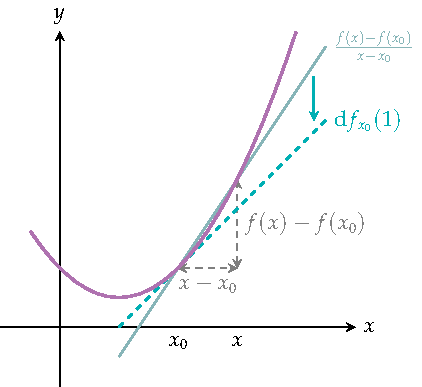
\includegraphics[width=0.7\textwidth]{figures/calculus/differential-definition.pdf}
\end{center}

我们将这些讨论整理为如下定义:

\begin{definition}[微分,导数]
    设$f:\R\to\R$,$x_0\in\R$,如果存在一个线性映射$\d f_{x_0}:\R\to\R$,使得
    \[
        f(x)=f(x_0)+\d f_{x_0}(x-x_0)+o(x-x_0),
    \]
    则称$f$在$x_0$处\textbf{可微}或者\textbf{可导},$\d f_{x_0}$是$f$在$x_0$处的\textbf{微分}. 微分具有形式$\d f_{x_0}(x)=kx$,其中$k$称为$f$在$x_0$处的\textbf{导数},记作$f'(x_0)$.

    如果$f$在$\R$的每一点都可微,则称$f$是\textbf{可微}的或者\textbf{可导}的,$\d f$是$f$的\textbf{微分},$f'$是$f$的\textbf{导(函)数},也记作$\frac{\d f}{\d x}$或$\dot{f}$.
\end{definition}

关于导数的符号有一些注. 最能体现几何意义的是$\frac{\d f}{\d x}$,它是由Leibniz发明的. 符号$\d$的意思就是“微”,可以理解为无穷小的变化量,所以导数就是自变量和函数值无穷小变化量的比值. 另一方面,这个符号也可以理解为“切”,表示切向量的意思,例如$\d x$就是沿着$x$轴的任意切向量(实际上就是正方向或者负方向),而$\d y$就是相应地沿着$y$轴的切向量. 从这个角度来说,$\frac{\d f}{\d x}$就是$x$轴切向量到$y$轴切向量的一个线性映射. 因此,微分其实就是所谓的\textbf{切映射},即切向量到切向量的映射. 这一视角在更抽象的微分学中是更本质的. 

导数的定义也可以用更常见的形式给出:

\begin{proposition}\label{prop:derivative}
    设$f:\R\to\R$,$x_0\in\R$,那么$f$在$x_0$处可微当且仅当如下极限存在:
    \[
        \lim_{x\to x_0}\frac{f(x)-f(x_0)}{x-x_0}.
    \]
    这个极限就是$f$在$x_0$处的导数. 因而,微分或者说导数是唯一的. 
\end{proposition}

下面我们不加证明地列举导数的一些性质,这些性质自然也导出了微分的性质. 

\begin{proposition}\label{prop:uni-derivative-property}
    设$f,g:\R\to\R$在$x_0$处可微,则
    \begin{itemize}
        \item $f$在$x_0$处连续;
        \item $(f+g)'(x_0)=f'(x_0)+g'(x_0)$;
        \item $(fg)'(x_0)=f'(x_0)g(x_0)+f(x_0)g'(x_0)$;
        \item 如果$g(x_0)\neq 0$,则
        \[\left(\frac{f}{g}\right)'(x_0)=\frac{f'(x_0)g(x_0)-f(x_0)g'(x_0)}{g(x_0)^2};\]
        \item 链式法则:如果$f$在$x_0$处可微,$g$在$f(x_0)$处可微,则$g\circ f$在$x_0$处可微,且$(g\circ f)'(x_0)=g'(f(x_0))f'(x_0)$;
        \item 如果$f$存在反函数$f^{-1}$,则$f^{-1}$在$f(x_0)$处可微,且$(f^{-1})'(f(x_0))=\frac{1}{f'(x_0)}$.
    \end{itemize}
\end{proposition}

在Leibniz记号下,如果$z=z(y)$,$y=y(x)$,那么链式法则可以写作
\[
    \frac{\d z}{\d x}=\frac{\d z}{\d y}\cdot\frac{\d y}{\d x}.
\]
反函数的导数则可以写作
\[
    \frac{\d y}{\d x}=\left(\frac{\d x}{\d y}\right)^{-1}.
\]
我们再次看到这种记号的天才之处,它将复杂的计算简化为了一种直观的形式.

我们指出,链式法则和反函数求导法则在微分下有更加清晰的含义:

\begin{proposition}\label{prop:derivative-geometric}
设$f:\R\to\R$在$x_0$处可微,$g:\R\to\R$在$f(x_0)$处可微,则
\begin{itemize}
    \item $\d x=\id$;
    \item $\d(g\circ f)_{x_0}=\d g_{f(x_0)}\circ\d f_{x_0}$.
    \item  如果$f$存在反函数$f^{-1}$,则$\d(f^{-1})_{f(x_0)}=(\d f_{x_0})^{-1}$.
\end{itemize}
\end{proposition}

\Cref{prop:derivative-geometric} 提供了这样一种视角:微分号$\d$相当于把$\R\to\R$的函数变成了另外一个$\R\to\R$的函数(即切映射),同时保持函数复合运算的单位元($\id$)、复合和逆元关系. 利用这一性质,我们可以用更加代数的方法研究微分(切函子),但这超出了本书的范围,我们就不再详细讨论了.

最后,我们讨论高阶导数的概念. 注意,我们只关注导数而不关注微分,这是因为由于高阶微分是一个相当抽象的概念,所以就不深入讨论了. 

\begin{definition}[高阶导数]
    设$f:\R\to\R$,$x_0\in\R$,如果$f$在$x_0$处可微,则$f$在$x_0$处的导数$f'(x_0)$是一个实数. 如果$f'$在$x_0$处可微,则称$f$在$x_0$处\textbf{二阶可微},此时$f''(x_0)$是$f'$在$x_0$处的导数,称为$f$在$x_0$处的\textbf{二阶导数}. 一般地,如果$f^{(n-1)}$在$x_0$处可微,则称$f$在$x_0$处\textbf{$n$阶可微},此时$f^{(n)}(x_0)$是$f^{(n-1)}$在$x_0$处的导数,称为$f$在$x_0$处的\textbf{$n$阶导数}.
\end{definition}
在Leibniz的记号下,$n$阶导数可以写作
\[
    \frac{\d^n y}{\d x^n}=\underbrace{\frac{\d}{\d x}\cdots\frac{\d}{\d x}}_{n\text{个}}y.
\]

从这里我们可以看出,$\d/\d x$这个记号又仿佛是一个算子,它作用在函数上,得到一个新的函数. 这个视角在谱理论中得到发扬,继而成为了量子力学的数学基础,用它可以证明矩阵力学和波动力学的等价性. 当然,这也不在本书的讨论范围之内了.

我们将在集合$X$上$n$次连续可微的函数(即$n$阶导数是连续函数)的集合记作$C^n(X)$,任意次连续可微的函数的集合记作$C^\infty(X)$. 在后面更一般的微分学中,$X$可以不是$\R$的子集,但我们依然沿用此记号,如果我们讨论的映射取值不在$\R$上,而是在抽象的集合$Y$上,我们将$C^n(X,Y)$记作从$X$到$Y$的$n$次连续可微映射的集合,$C^\infty(X,Y)$记作任意次连续可微的从$X$到$Y$的映射的集合,这些概念的定义将在后面给出. 

\subsection{微分学基本定理}

微分学几乎都与极值联系在一起,刻画这些关系的定理就是微分学的基本定理. 我们依然只罗列定理,不给出证明. 首先我们给出极值的定义. 

\begin{definition}[极大值,严格极大值,极小值,严格极小值]\label{def:extremum}
    设$f:X\to\R$,$x_0\in X$,如果存在包含$x_0$的开集$U$,使得对任意$x\in U$,有$f(x)\leq f(x_0)$,则称$f(x_0)$是$f$在$x_0$处的一个\textbf{极大值},$x_0$是$f$的一个\textbf{极大值点}. 如果$f(x)=f(x_0)$只在$x_0$处成立,则称$f(x_0)$是$f$在$x_0$处的一个\textbf{严格极大值},$x_0$是$f$的一个\textbf{严格极大值点}.
    
    如果不等式反向,则称$f(x_0)$是$f$在$x_0$处的一个\textbf{极小值},$x_0$是$f$的一个\textbf{极小值点}. 如果$f(x)=f(x_0)$只在$x_0$处成立,则称$f(x_0)$是$f$在$x_0$处的一个\textbf{严格极小值},$x_0$是$f$的一个\textbf{严格极小值点}.
    
    如果$f(x_0)$是$f$在$x_0$处的一个极大(小)值,则称$f(x_0)$是$f$在$x_0$处的一个\textbf{极值},$x_0$是$f$的一个\textbf{极值点}. 
\end{definition}

首先是Fermat引理,他其实就是极值的一阶必要条件:

\begin{lemma}[Fermat引理]\label{lemma:fermat}
    设$f:X\to\R$,$x_0\in X$是$f$的一个极值点,且$f$在$x_0$处可微,则$f'(x_0)=0$.
\end{lemma}

接下来是一系列中值定理,我们这里只给出Lagrange中值定理:

\begin{theorem}[Lagrange中值定理]\label{thm:lagrange-mid}
    设$f:[a,b]\to\R$是一个连续函数,且在$(a,b)$内可微,则存在$\xi\in(a,b)$,使得
    \[
        f'(\xi)=\frac{f(b)-f(a)}{b-a}.
    \]
\end{theorem}

这一定理给出了割线斜率和切线斜率的关系,可以用下图来理解:

\begin{center}
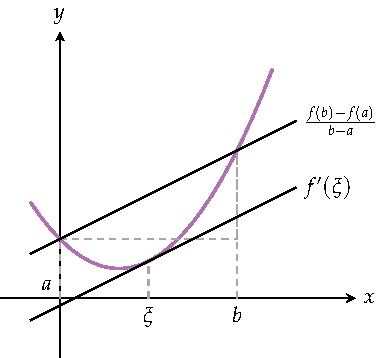
\includegraphics[width=0.6\textwidth]{figures/calculus/Lagrange.pdf}
\end{center}

我们将在后面指出,这一定理只适用于实值函数,假如想对向量值函数使用,需要对其进行适当的修改:

\begin{theorem}[Lagrange有限增量定理]\label{thm:lagrange-finite}
    设$f:[a,b]\to\R$是一个连续函数,且在$(a,b)$内可微,则
    \[
        |f(b)-f(a)|\leq |b-a|\sup_{\xi\in(a,b)}|f'(\xi)|.
    \]
\end{theorem}

接下来我们讨论高阶导数与极值的关系. 这样的关系是由Taylor公式给出的. 我们说过,微分是用线性函数去近似函数的过程,而Taylor公式则是用多项式去近似函数的过程. 考虑函数$f:\R\to\R$,如果$f$在$x_0$处$n$次可微,我们尝试用一个$n$次多项式去近似$f$,即

\[
    f(x)=a_0+a_1(x-x_0)+\cdots+a_n(x-x_0)^n+o((x-x_0)^n).
\]
容易求出,$a_0=f(x_0)$,$a_1=f'(x_0)$,$a_2=\frac{f''(x_0)}{2}$,$a_3=\frac{f'''(x_0)}{6}$,$\cdots$,$a_k=\frac{f^{(k)}(x_0)}{k!}$,因此我们得到了Taylor公式:

\begin{theorem}
    设$f:\R\to\R$在$x_0$处$n$次可微,则
    \[
        f(x)=\sum_{k=0}^n\frac{f^{(k)}(x_0)}{k!}(x-x_0)^k+o((x-x_0)^n).
    \]
\end{theorem}

我们将这个$n$次多项式称为\textbf{Taylor展开}.

利用Taylor展开,我们可以得到通过高阶导数判定极值的充分条件:

\begin{theorem}\label{thm:extreme}
    设$f:(a,b)\to\R$在$x_0$处$n$次可微,且$f'(x_0)=f''(x_0)=\cdots=f^{(n-1)}(x_0)=0$,$f^{(n)}(x_0)\neq 0$,则
    \begin{itemize}
        \item 如果$n$为奇数,$f$在$x_0$处没有极值;
        \item 如果$n$为偶数,$f$在$x_0$处有极值,且当$f^{(n)}(x_0)>0$时,$f$在$x_0$处有严格极小值,当$f^{(n)}(x_0)<0$时,$f$在$x_0$处有严格极大值.
    \end{itemize}
\end{theorem}

\section{多元函数的微分学}

这一部分讨论$\R^n\to\R^m$的微分学,当$m=1$,我们称之为实值函数;对一般的$m$,我们称之为向量值函数. 这一部分需要很多线性代数的知识,请参阅\Cref{chap:linear-algebra}.

\subsection{微分、偏导数与导数的定义}\label{subsec:partial-derivative}

沿着一元函数的思路,我们希望找到一个线性映射$df_x:\R^n\to\R^m$,使得$f$在$x$附近的行为很接近这个线性映射,而这件事情本身就可以作为微分的定义:

\begin{definition}[微分]
    设$f:\R^n\to\R^m$,$x\in\R^n$,如果存在一个线性映射$\d f_{x}:\R^n\to\R^m$,使得
    \[
        f(x+h)=f(x)+\d f_{x}h+o(h),
    \]
    则称$f$在$x_0$处\textbf{可微}或者\textbf{可导},$\d f_{x_0}$是$f$在$x_0$处的\textbf{微分}. 这里$o(h)$理解为一个向量值函数$\alpha:\R^n\to\R^m$,它满足$\lim_{h\to 0}\norm{\alpha(h)}/\norm{h}=0$\footnote{在\Cref{ex:lp-topology} 中我们提到过,$L^p$范数下的$\R^n$的拓扑都是一样的. 但是,为了利用内积的性质,之后我们写出符号$\norm{\cdot}$的时候,都指$L^2$范数.}.

    如果$f$在$\R^n$的每一点都可微,则称$f$是\textbf{可微}的或者\textbf{可导}的,$\d f$是$f$的\textbf{微分}.
\end{definition}

现在我们来解释这一定义的含义. 微分的定义依然是将一个关于$x$的函数转变到一个关于$h$的线性映射,这个线性映射表明了函数在$x$处的线性近似,而这个线性近似的误差是一个关于$h$的高阶无穷小. 从这个角度来说,微分的定义和一元函数的情况是一样的,只不过这里的误差是一个向量值函数而已. 

$h$被称为\textbf{切向量}(回忆一维的情况),所有允许$h$的集合记为$T\R_x^n$,称为在$x$点处的\textbf{切空间}. $\R^n$上定义的函数,切向量$h$自然可以取遍所有$\R^n$的向量,所以其实$T\R_x^n=\R^n$. 然而在\Cref{chap:duality}中,我们会看到,当定义域不是整个$\R^n$,而只是某个子集的时候,切空间的定义就变得不平凡了. 从“切”的视角来看,微分其实是一个\textbf{切映射},即从切向量到切向量的映射,这可以用下图来表示:

\[\begin{tikzcd} f:\arrow[mapsto, d, "\d"] & \R^n\arrow[r, ""] & \R^m \\
\d f_x: & T\R^n_x \arrow[r, ""] & T\R^m_{f(x)}
\end{tikzcd}\]

接下来的问题就是,如何表示线性映射$\d f_x$?我们先从实值函数开始. 考虑$\R^n$的标准正交基$\{e_i\}_{i=1}^n$,它也是切空间$T\R^n_x$的标准正交基,根据Riesz表示定理(\Cref{thm:riesz}),存在一个向量$g$,使得
\[
    \d f_x h=\inner{g}{h}.
\]
这个向量$g$被称为$f$在$x$处的\textbf{梯度},记作$\grad f(x)$. 

我们需要进一步将梯度的坐标$(g_1,\dots,g_n)^\t$求出来. 考虑一个具体的分量$e_i$,根据定义,
\[f(x+te_i)=f(x)+t\d f_x(te_i)+o(te_i)=f(x)+g_it+o(t).\]
因此,
\[g_i=\lim_{t\to 0}\frac{f(x+te_i)-f(x)}{t}.\]
我们给这样的导数一个名字,称为$f$在$x$对$x_i$的\textbf{偏导数},记作$\frac{\partial f}{\partial x_i}(x)$或$\partial_i f(x)$,于是我们得到了梯度的坐标:
\[\left(\frac{\partial f}{\partial x_1}(x),\dots,\frac{\partial f}{\partial x_n}(x)\right)^\t.\]

当然,我们不一定要沿着$e_i$去算导数,我们可以沿着任意单位向量$u$去算,于是我们得到了$f$在$x$处沿着$u$的\textbf{方向导数}:
\[\frac{\partial f}{\partial u}(x)=\lim_{t\to 0}\frac{f(x+tu)-f(x)}{t},\quad\norm{u}=1.\]

有了梯度,我们可以很快算出任意方向导数:

\begin{proposition}\label{prop:directional-derivative}
    设$f:\R^n\to\R$在$x$处可微,$u$是单位向量,则
    \[\frac{\partial f}{\partial u}(x)=\inner{\grad f(x)}{u}.\]
\end{proposition}

在微积分中,我们总是假设在标准正交基下进行计算,在这种情况下,我们有更简便的表示方式. 形式上,记
\[\nabla =e_1\frac{\partial }{\partial x_1}+\cdots+e_n\frac{\partial }{\partial x_n},\]
则
\[\grad f(x)=\nabla f(x).\]
符号$\nabla$被称为\textbf{nabla算子},它就是标准正交基下梯度的具体表示. 通常,我们会更简单地将$\nabla $记为$(\partial_1 ,\dots,\partial_n)^\t$. 

接下来我们讨论向量值函数微分的表示问题. 选取$\R^m$(也就是$T\R_x^n$)的标准正交基$e_i$,选取$\R^m$(也就是$T\R^m_{f(x)}$)的标准正交基$e_i$,则根据\Cref{sec:matrix}的讨论,我们可以用一个$m\times n$的矩阵来表示$\d f_x$,这个矩阵被称为$f$在$x$处的\textbf{Jacobi矩阵},记作$J_f(x)$. 

下面我们计算$J_f(x)$的具体表示. 假设$f(x)$的坐标是$(f_1(x),\dots,f_m(x))^\t$,考虑$h\in T\R_x^n$,它的坐标是$(h_1,\dots,h_n)^\t$,$\d f_x h$的坐标应该是
\[\begin{pmatrix}
    \d f_{1,x}h \\
    \vdots \\
    \d f_{m,x}h
\end{pmatrix}=
\begin{pmatrix}
    \sum_{i=1}^n\partial_i f_1(x)h_i \\
    \vdots \\
    \sum_{i=1}^n\partial_i f_m(x)h_i
\end{pmatrix}=
\begin{pmatrix}
    \partial_1 f_1(x) & \cdots & \partial_n f_1(x) \\
    \vdots & \ddots & \vdots \\
    \partial_1 f_m(x) & \cdots & \partial_n f_m(x)
\end{pmatrix}
\begin{pmatrix}
    h_1 \\
    \vdots \\
    h_n
\end{pmatrix}.\]
因此,我们得到了Jacobi矩阵:
\[J_f(x)=(\partial_j f_i)=\begin{pmatrix}
    \partial_1 f_1(x) & \cdots & \partial_n f_1(x) \\
    \vdots & \ddots & \vdots \\
    \partial_1 f_m(x) & \cdots & \partial_n f_m(x)
\end{pmatrix}.\]

在$m=n$的特殊情况下,$J_f(x)$的行列式被称为$f$在$x$处的\textbf{Jacobi行列式},记作
\[\frac{\partial(f_1,\dots,f_n)}{\partial(x_1,\dots,x_n)}(x).\]
在\Cref{ex:polar-coordinates} 中我们会看到,Jacobi行列式表明了坐标变换时相应体积变化的比率. 这一事实使得它在积分学的变量替换中有着核心作用. 

总结来说,实值函数的微分可以用\textit{行}向量$(\partial_1 f_1(x),\dots,\partial_n f_1(x))$和切向量相乘表示,而向量值函数的微分可以用Jacobi矩阵$J_f(x)$和切向量相乘来表示,我们将这些符号统称$f$在$x$处的\textbf{导数},记为$f'(x)$或$\frac{\d f}{\d x}(x)$,于是,在坐标表示下,我们可以将微分简单写作$\d f_x=f'(x)\d x$,这里我们将$\d x$理解为一个切向量(列向量). 

接下来,我们不加证明地列举微分的一些性质:

\begin{proposition}\label{prop:derivative-property}
    设$f,g:\R^n\to\R^m$在$x$处可微,则
    \begin{itemize}
        \item $f$在$x$处连续;
        \item 对任意$\lambda_1,\lambda_2\in\R$, $\d(\lambda_1 f_x+\lambda_2 g_x)=\lambda_1\d f_x+\lambda_2\d g_x$;
        \item 如果$m=1$,那么$\d(f\cdot g)_x=g(x)\d f_x+f(x)\d g_x$;
        \item 如果$m=1$,并且$g(x)\neq 0$,则
        \[\d\left(\frac{f}{g}\right)_x=\frac{1}{g(x)^2}\left(g(x)\d f_x-f(x)\d g_x\right);\]
        \item 如果$m=n$,那么$\d x=\id$;
        \item 链式法则:如果$f$在$x$处可微,$g$在$f(x)$处可微,则$g\circ f$在$x$处可微,且$\d(g\circ f)_x=\d g_{f(x)}\circ\d f_x$;
        \item 如果$f$存在反函数$f^{-1}$,则$f^{-1}$在$f(x)$处可微,且$\d(f^{-1})_{f(x)}=(\d f_x)^{-1}$.
    \end{itemize}
\end{proposition}

同样,最后三条说明了微分保持了复合单位元、复合和逆元关系. 而第二条则说明微分是一个函数空间($\R^n\to\R^m$)到函数空间($T\R_x^n\to T\R^m_{f(x)}$)的线性映射.

链式法则与反函数求导法则可以用导数写出:
\[(f\circ g)'(x)=f'(g(x))g'(x),\quad (f^{-1})'(f(x))=(f'(x))^{-1}.\]
这里我们都将导数理解为矩阵. 同样,在Leibniz记号下,如果$z=z(y)$,$y=y(x)$,那么链式法则可以写作
\[
    \frac{\d z}{\d x}=\frac{\d z}{\d y}\cdot\frac{\d y}{\d x}.
\]
反函数的导数则可以写作
\[
    \frac{\d y}{\d x}=\left(\frac{\d x}{\d y}\right)^{-1}.
\]
他们的含义都非常清晰. 


我们看几个重要的例子. 

\begin{example}\label{ex:linear-derivative}
线性映射和线性函数本身的导数也非常简单:
\[\frac{\d (Ax)}{\d x}=A,\quad \frac{\d (b^\t x)}{\d x}=b^\t.\]
其中$A$是一个矩阵,$b$是一个向量. 
\end{example}

\begin{example}
    考虑一个多元实值函数$g(x)=f(u_1(x),\dots,u_k(x))$,先求$f$对$u=(u_i)$的导数:
    \[\frac{\d f}{\d u}=\left(\frac{\partial f}{\partial u_1},\dots,\frac{\partial f}{\partial u_k}\right).\]
    再求$u$对$x$的导数$\d u/\d x=(u_1'(x),\dots,u_k'(x))^\t$. 根据链式法则,
    \[\frac{\d g}{\d x}=\frac{\d f}{\d u}\cdot\frac{\d u}{\d x}=\left(\frac{\partial f}{\partial u_1},\dots,\frac{\partial f}{\partial u_k}\right)\begin{pmatrix}
        u_1'(x) \\
        \vdots \\
        u_k'(x)
    \end{pmatrix}=\sum_{i=1}^k\frac{\partial f}{\partial u_i}u_i'(x).\]
\end{example}

\begin{example}
我们来看一个更复杂的例子,这个例子可以表明所谓\textit{求导链}的意义. 考虑函数$f(x,y,z)=z\exp(x+y)$,其中$z(x,y)=x+y$. 我们来求$f$对$x$的偏导数. 首先,我们把变量之间的依赖关系用如下图表示出来,其中$z\to y$表示$z$依赖$y$.
\begin{center}
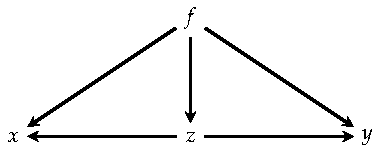
\includegraphics[width=0.55\textwidth]{figures/calculus/back-propagation.pdf}
\end{center}
我们要求$f$对$x$的偏导数,首先找到从$f$出发可以到达$x$的全部路径,即$f\to z\to x$和$f\to x$,然后将路径上的相邻变量的偏导数相乘再相加,即
\[\frac{\partial f}{\partial x}=\frac{\partial f}{\partial z}\cdot\frac{\partial z}{\partial x}+\frac{\partial f}{\partial x}=\exp(x+y)\cdot 1+z\exp(x+y).\]
这里两边都出现了$\partial f/\partial x$,但他们的含义是不同的,左边的$\partial f/\partial x$是$f$对$x$这个变量的偏导数,右边的$\partial f/\partial x$是$f$对第一个位置偏导数,即$\partial_1 f$. 一个不容易引起困惑但不太直观的写法是
\[\frac{\partial f}{\partial x}=\partial_3 f\cdot\partial_1 z+\partial_1 f.\]

这就是著名的\textbf{反向传播算法}的一个简单例子,它是神经网络训练中最重要的算法之一,也是很多神经网络框架优化的重点. 
\end{example}

\begin{example}\label{ex:quadratic-derivative}
考虑二次型$f(x)=x^\t A x$(因此假设$A$是对称矩阵),我们来求$f'(x)$. 为此,考虑一个新函数$g(x,y)=x^\t A y$,则$f(x)=g(x,x)$,于是

\[f'(x)=g'(x,x)=\partial_1 g(x,x)\cdot\frac{\partial x}{\partial x}+\partial_2 g(x,x)\cdot\frac{\partial x}{\partial x}=\partial_1 g(x,x)+\partial_2 g(x,x).\]

我们来计算$\partial_1 g(x,x)$,$g(x,y)=(Ay)^\t x$,因此根据\Cref{ex:linear-derivative},$\partial_1 g(x,y)=(Ay)^\t$,于是$\partial_1 g(x,x)=x^\t A^\t$,同理$\partial_2 g(x,x)=x^\t A$,因此$f'(x)=x^\t A+x^\t A^\t=(2Ax)^\t$.
\end{example}

\begin{remark}
在求向量对向量的导数的时候,很容易搞不清楚Jacobi矩阵的行列顺序,一个简单的检查方法是看看导数的维度是否正确,例如我们可以试试这一个矩阵是否可以乘自变量,然后得到因变量的维数,例如\Cref{ex:quadratic-derivative} 中,如果我们求出来导数是$2Ax$,那么$2Axx$是一个无意义的量,说明我们的导数求错了,应该要进行转置. 

矩阵行列如何排列其实不影响导数值,但是在进行链式法则的时候,正确的排列可以机械地写出链式法则的结果,这样才能实现自动求导器. 
\end{remark}

最后,我们讨论高阶导数的概念. 对于向量值函数来说,高阶导数是一个非常难以理解的概念,所以我们只局限在实值函数讨论这一问题. 

考虑一个实值函数$f:\R^n\to\R$,它对第$i$个坐标的偏导数是$\partial_i f$,注意到这本身又是一个$\R^n$到$\R$实值函数,我们可以继续讨论它的偏导数性质,于是我们得到了\textbf{二阶偏导数}:$\partial_j(\partial_i f)$,也记为
\[\frac{\partial^2 f}{\partial x_j\partial x_i},\quad\partial_{j,i} f(x).\]

一般地,我们也可以归纳定义$k$阶偏导数,这里就不再赘述. 

二阶偏导数一个重要的性质是,一般情况下它可交换求偏导的顺序:

\begin{proposition}\label{prop:partial-commute}
    设$f:\R^n\to\R$具有下列两个二阶偏导数
    \[\frac{\partial^2 f}{\partial x_j\partial x_i}(x),\frac{\partial^2 f}{\partial x_i\partial x_j}(x),\]
    并且在$x$处他们都连续,则两个偏导数相等.
\end{proposition}

一个直接的推论是,对于$C^k(X)$的函数来说,求$k$阶偏导数不依赖于求导的顺序. 

我们来看一个重要的例子. 
\begin{example}\label{ex:multi-taylor}
设函数$f\in C^k(\R^n)$,$x,h\in\R^n$,考虑$g(t)=f(x+th)$,$t\in[0,1]$,我们来求$g^{(m)}(t)$,其中$m\leq k$. 先求一阶导数,根据链式法则,
\[g'(t)=\sum_{i=1}^n\partial_i f(x+th)h_i.\]
利用nabla算子,我们可以写作$g'(t)=(h^\t\nabla) f$.
再求二阶导数,根据\Cref{prop:partial-commute} 和链式法则,
\[g''(t)=\sum_{i=1}^nh_i\frac{\d}{\d t}(\partial_i f(x+th))=\sum_{i=1}^nh_i\sum_{j=1}^n\partial_j(\partial_i f(x+th))h_j=\sum_{i,j=1}^nh_ih_j\partial_{j,i}f(x+th).\]
用nabla算子,我们可以写作$g''(t)=(h^\t\nabla)^2f(x+th)$. 一般地,我们有
\[g^{(m)}(t)=\sum_{i_1,\dots,i_m}\partial_{i_m,\dots,i_1}f(x+th)h_{i_1}\cdots h_{i_m}=(h^\t\nabla)^mf(x+th).\]
\end{example}

接下来,我们定义二阶导数\footnote{更高阶的导数定义需要更加复杂的线性代数概念,我们这里就不引入了. }. 注意到,一个实值函数的一阶导数可以表示成一个向量值函数,即$\grad f$,因此,这个向量值函数的导数就是一个矩阵. 我们将这个矩阵称为$f$的\textbf{Hessian矩阵},记作$H_f(x)$. 很容易算出,Hessian矩阵为
\[H_f(x)=\begin{pmatrix}
    \partial_{1,1}f(x) & \cdots & \partial_{1,n}f(x) \\
    \vdots & \ddots & \vdots \\
    \partial_{n,1}f(x) & \cdots & \partial_{n,n}f(x)
\end{pmatrix}.\]

显然,Hessian矩阵是一个对称矩阵,因而可以构成某个二次型. \Cref{ex:multi-taylor} 中二阶导数其实已经暗示了这一点,我们可以将二阶导数写成一个二次型的形式:
\[g''(t)=h^\t H_f(x+th)h.\]

\subsection{微分学基本定理}

类似一元函数,我们讨论极值与导数的关系,我们也不给出具体证明. 注意,一元函数的极值的定义(\Cref{def:extremum})已经包含了多元函数情形,所以这里就不再重复. 

首先是Fermat引理的推广:

\begin{lemma}[Fermat引理]\label{lemma:fermat-multi}
    设$f:\R^n\to\R$,$x_0\in\R^n$是$f$的一个极值点,且$f$在$x_0$处可微,则$f'(x_0)=0$.
\end{lemma}

接下来是一系列中值定理,我们这里依然只给出Lagrange中值定理:

\begin{theorem}[Lagrange中值定理]\label{thm:lagrange-mid-multi}
    设$f:\R^n\to\R$是一个实值函数,在闭区间$[x,x+h]=\{x+th:t\in[0,1]\}$上连续,开区间$(x,x+h)=\{x+th:t\in(0,1)\}$上可微,则存在$\xi\in(x,x+h)$,使得
    \[
        f(x+h)-f(x)=f'(\xi)h.
    \]
\end{theorem}
用参数的形式,$\xi$可以写作$\xi=x+\theta h$,其中$\theta\in(0,1)$.

接下来我们讨论向量值函数的中值定理. 下面的例子表明,向量值函数上中值定理不一定成立:
\begin{example}
考虑匀速圆周运动,$r(t)=(\cos t,\sin t)$,它的速度向量是$r'(t)=(-\sin t,\cos t)$. 当绕一个周期之后,位置又回到了原点,于是$r(2\pi)-r(0)=0$,然而$r'(t)$恒不为$0$,因此不存在$\xi\in(0,2\pi)$使得$r(2\pi)-r(0)=r'(\xi)(2\pi-0)$.
\end{example}

不过,中值定理的弱化版本,有限增量定理,是成立的:

\begin{theorem}[Lagrange有限增量定理]\label{thm:lagrange-finite-multi}
    设$f:\R^n\to\R^m$是一个函数,在闭区间$[x,x+h]$上连续,开区间$(x,x+h)$上可微,则
    \[
        \norm{f(x+h)-f(x)}\leq \norm{h}\sup_{\xi\in(x,x+h)}\norm{f'(\xi)}.
    \]
\end{theorem}

注意,这里的$f'(\xi)$可能是一个矩阵,此时$\norm{f'(\xi)}$的含义是矩阵范数,具体的讨论参见\Cref{sec:operator-norm}. 

\begin{example}\label{ex:lagrange-finite-multi}
这个例子探讨如何用二阶导数控制一阶导数的变化. 这一部分需要算子范数和谱理论的知识,请参阅\Cref{sec:operator-norm}. 

假设$f\in C^2(X)$,$X\subseteq\R^n$,那么对任意$x,y\in X$满足$[x,y]\in X$,根据\Cref{thm:lagrange-finite-multi} 和Hessian矩阵的定义,我们有
\[\norm{\grad f(x)-\grad f(y)}\leq \norm{x-y}\sup_{\xi\in(x,y)}\norm{H_f(\xi)}.\]

我们讨论两种情况,首先假设$X$是紧集. 因为$H_f(x)$连续,根据\Cref{ex:metric-norm-continuous},$\norm{\cdot}$连续,再根据\Cref{prop:continuous-composition},$\norm{H_f(x)}$连续. 由于$X$是紧集,根据Weierstrass最值定理(\Cref{thm:weierstrass})$\norm{H_f(x)}$在$X$上取到最大值$M$,因此,我们有
\[\norm{\grad f(x)-\grad f(y)}\leq M\norm{x-y}.\]

这一推导表明紧集上的$C^2$函数的梯度是\textit{Lipschitz连续}的. 所谓$F$是Lipschitz连续的,指的是存在一个常数$M$,使得对于任意定义域里的$x,y$,我们都有$\norm{F(x)-F(y)}\leq M\norm{x-y}$. 

在第二种情况下,假设$X=\R^n$,我们使用$L^2$范数,于是根据\Cref{thm:symmetric-operator-norm},我们有
\[\norm{\grad f(x)-\grad f(y)}\leq\sup_{\lambda\in\sigma(H_f(z)),z\in(x,y)}|\lambda|\cdot \norm{x-y}.\]
这里$\sigma(A)$是矩阵$A$的谱. 

因此,只要知道了Hessian矩阵的谱,我们就可以控制梯度的变化,这一点对于凸优化算法非常重要,具体讨论见\Cref{ex:gradient-descent}.
\end{example}

最后,我们要讨论高阶导数与极值的关系. 首先,利用\Cref{ex:multi-taylor} 和一元的Taylor公式,我们可以得到多元函数的Taylor公式:

\begin{theorem}[Taylor展开]
    设$f\in C^k(U)$,$[x,x+h]\subseteq U$,那么
    \[
        f(x+h)=\sum_{j=0}^k\frac{1}{j!}(h^\t\nabla)^jf(x)+o(\norm{h}^k).
    \]
\end{theorem}

根据这一定理,我们可以得到二阶导数判定极值的充分条件:

\begin{theorem}\label{thm:second-derivative-test}
    设$f\in C^2(U)$,$U$是开集,$x_0\in U$且$f'(x_0)=0$,则
    \begin{itemize}
        \item 如果$H_f(x_0)$是正定的,则$f$在$x_0$处取极小值;
        \item 如果$H_f(x_0)$是负定的,则$f$在$x_0$处取极大值;
        \item 如果$H_f(x_0)$不定(既非半正定也非半负定),则$f$在$x_0$处不取极值.
    \end{itemize}
\end{theorem}

\subsection{隐函数定理}

微积分中,还有一类非常重要的问题,那就是解方程,我们看一个非常简单的例子. 设$f:\R^2\to\R$,$f(x,y)=x^2+y^2-1$,我们来求解方程$f(x,y)=0$,也就是求单位圆的方程. 由于$f$是一个二次型,因此我们可以直接求出它的根:
    \[y=\pm\sqrt{1-x^2}.\]
比如考虑圆周上的点$(0.6,0.8)$的附近,$x$就可以把$y$表示出来:$y=\sqrt{1-x^2}$. 如果考虑点$(0.6,-0.8)$的附近,我们也可以写出$y=-\sqrt{1-x^2}$. 
    
总而言之,只要给定圆周上一个点$(x_0,y_0)$($y_0\neq 0$),我们就可以找到一个邻域,在这个邻域上确认一个$y$和$x$的函数关系$y=y(x)$.

更一般地,给定函数方程$F(x,y)=0$,它确定了一个平面上的曲线$C=\{(x,y)\in\R^2:F(x,y)=0\}$. 任取一点$(x_0,y_0)\in C$,如果在$(x_0,y_0)$的某个邻域$U$上,我们可以确认一个$y$和$x$的函数关系$y=y(x)$,使得$U\cap C$中的所有点都可以用这个关系表示,那么我们其实就把一个隐藏在$F(x,y)=0$中的函数$y$解出来了,这就是\textbf{隐函数}的概念.

下面,我们考虑维数更高的情况. 设$F:\R^n\times\R^m\to\R^k$,$F(x,y)=0$,其中$x\in\R^n$,$y\in\R^m$. 任取一点$(x_0,y_0)$满足$F(x_0,y_0)=0$,同样,我们希望在$(x_0,y_0)$的某个邻域$U$上,将$F(x,y)=0$转化为一个等价的函数关系$y=y(x)$. 

首先我们指出,在一般情况下,$k=m$的时候讨论才有意义,这可以从线性方程组的理论看出,相关的线性代数理论可以参见\Cref{chap:linear-algebra}. 假如说$F(x,y)=0$就是一个线性方程组:
\begin{equation}
    \begin{gathered}
        a_{11}x_1+\cdots+a_{1n}x_n+b_{11}y_1+\cdots+b_{1m}y_m-c_1=0, \\
        \dots \\
        a_{k1}x_1+\cdots+a_{kn}x_n+b_{k1}y_1+\cdots+b_{km}y_m-c_k=0.
    \end{gathered}
    \label{eq:linear-equation}
\end{equation}
我们也可以写成矩阵形式:
\[Ax+By=c.\]
其中$A$是一个$k\times n$的矩阵,$B$是一个$k\times m$的矩阵,$c$是一个$k$维向量.

如果$k<m$,那么线性映射$y\mapsto By$的秩是$k<m$,根据\Cref{cor:kernel-image-isomorphism},这个映射的核不是$\{0\}$,所以对于任意一个满足$Ax_0+By_0=c$的$(x_0,y_0)$来说,总可以再加上一个$y\neq 0$使得$Ax_0+B(y+y_0)=c$且$\norm{y}$充分小. 因此对任何$x_0$,都找不到一个$y$的邻域,其中有唯一的$y$使得$Ax_0+By=c$,所以我们也不能解出$y=y(x)$.

如果$k>m$,那么$F(x,y)=0$很有可能是空集. 比如,下列线性方程组就没有解:
\begin{gather*}
    x_1+x_2=0, \\
    x_1+x_2=1.
\end{gather*}

对于非线性方程组的情况,如果$F(x,y)$是可微的,那么在一个点的局部函数的性质可以用线性映射近似,于是也应该有$k=m$. 这一事实可以简单归结为:\textit{要解$m$个未知数(即$y$),应该恰好有$m$个方程(即$F(x,y)=0$)}.

我们继续来看线性方程组的情况,即 \eqref{eq:linear-equation},如果$k=m$,$c=0$,$B$可逆,很快就可以解出
\[y=-B^{-1}Ax.\]

对于一般的$F$,在它的每一个局部,我们都可以用一个线性映射近似,根据微分的偏导数表示,这一线性映射恰好形如
\[\underbrace{\frac{\partial F}{\partial x}}_A h_x+\underbrace{\frac{\partial F}{\partial y}}_B h_y.\]
这里$h_y$和$h_x$就应该理解为映射在这一点的切向量. 
于是,假如$\frac{\partial F}{\partial y}$可逆,那么我们就可以解出
\[h_y=-\left(\frac{\partial F}{\partial y}\right)^{-1}\frac{\partial F}{\partial x}h_x.\]
假设我们可以解出函数关系$y=f(x)$,由于$h_x$和$h_y$是切向量,根据导数的定义,
\[f'(x)=-\left(\frac{\partial F}{\partial y}\right)^{-1}\frac{\partial F}{\partial x}.\]

确定了导数就可以确定这个函数本身,这就是\textbf{隐函数定理}的内容. 下面,我们正式给出它的陈述. 

\begin{theorem}[隐函数定理]\label{thm:implicit-function}
    设$F:\R^n\times\R^m\to\R^m$,$F(x,y)=0$,其中$x\in\R^n$,$y\in\R^m$,考虑点$(x_0,y_0)$的邻域$U$,如果:
    \begin{itemize}
        \item $F\in C^p(U;\R^m)$,$p\geq 1$;
        \item $F(x_0,y_0)=0$;
        \item $\frac{\partial F}{\partial y}(x_0,y_0)$可逆,
    \end{itemize}
    那么存在开球$B(x_0,r)\subseteq\R^n$,开球$B(y_0,s)\subseteq\R^m$,以及一个函数$f\in C^p(B(x_0,r);\R^m)$,使得对任意$x\in B(x_0,r)$,$y\in B(y_0,s)$,都有
    \[F(x,y)=0\iff y=f(x).\]
    此外,$f$的导数可以用$F$的偏导数表示:
    \[f'(x)=-\left(\frac{\partial F}{\partial y}\right)^{-1}\frac{\partial F}{\partial x}.\]
\end{theorem}

用Banach不动点定理(\Cref{thm:banach-fixed-point}),我们可以给一个该定理的简洁证明,具体内容请参见\Cref{chap:fixed-point-theory}的习题\Cref{???}. 

隐函数定理的一个特例是向量值函数的反函数的存在性定理:

\begin{theorem}[反函数定理]\label{thm:inverse-function}
    设$f\in C^p(\R^n;\R^n)$,$p\geq 1$,$f'(x_0)$可逆,那么存在$x_0$的邻域$V$,以及$f(x_0)$的邻域$W$,使得$f:V\to W$是一个双射,且$f^{-1}\in C^p(W;\R^n)$,此外,$f^{-1}$的导数可以用$f$的导数表示,对于$x\in V,y=f(x)\in W$,我们有
    \[f^{-1}(y)'=(f'(x))^{-1}.\]
\end{theorem}

作为一个注,反函数定理中可逆性的判断可以利用Jacobi行列式是否非零来判断. 

反函数定理最重要的用途是坐标变换. 我们之前的坐标变换都是线性的基到线性的基,然而在微积分中\textit{非线性}的坐标也非常常用,比如极坐标、球坐标等. 这些坐标变换都是非线性的,因此我们需要反函数定理来处理这些坐标变换. 我们考虑极坐标的例子. 

\begin{example}[极坐标]\label{ex:polar-coordinates}
    考虑一个半平面$\R_{\geq 0}\times\R=\{(r,\phi)\in\R\times\R:r\geq 0\}$. 我们将它映射到$\R^2$平面上,映射$f$定义为$f(r,\phi)=(r\cos\phi,r\sin\phi)$. 我们也可以写得更像坐标变换一些:
    \begin{gather*}
        x=r\cos\phi, \\
        y=r\sin\phi.
    \end{gather*}
    这个变换的Jacobi行列式是$r$,因此除了$r=0$的点,这个变换都是可逆的,于是在$\R^2$的任何局部上,我们都可以用极坐标来表示平面上的点.

    我们借着这个例子来看一下Jacobi行列式的几何意义. 上述坐标变换的微分是:
    \[\begin{pmatrix}
        \d x \\
        \d y
    \end{pmatrix}=\begin{pmatrix}
        \cos\phi & -r\sin\phi \\
        \sin\phi & r\cos\phi
    \end{pmatrix}\begin{pmatrix}
        \d r \\
        \d\phi
    \end{pmatrix}=J_f \begin{pmatrix}
        \d r \\
        \d\phi
    \end{pmatrix}.\]

    这里对诸如$\d x$的符号,我们有两种理解方式,一种是把他们理解为切向量,另一种是把他们理解为一段微小位移. 不论哪一种,最终结果都是将$f$在局部近似为了一个线性映射. 根据\Cref{sec:determinant} 的讨论,这一线性映射将平行体$\Pi(\d r,\d \phi)$映射为平行体$\Pi(\d x,\d y)$,而Jacobi行列式就是他们有向体积变化的比率. 如果我们把$\Pi(\d r,\d \phi)$的有向体积记为$\partial(r,\phi)$,那么我们有
    \[\frac{\partial(x,y)}{\partial(r,\phi)}=\det J_f.\]
    这正是Jacobi行列式这一符号的意义. 
    
    我们还可以用Leibniz的记号更加形象地表达这件事情. 作为坐标,我们认为$\d x\d y$表示的正好就是长方形$\Pi(\d x,\d y)$的有向面积(长乘宽),而$\d r\d\phi$表示的正好就是长方形$\Pi(\d r,\d \phi)$的有向面积,于是我们有
    \[\frac{\d x\d y}{\d r\d\phi}=\frac{\partial(x,y)}{\partial(r,\phi)}\iff \d x \d y= \frac{\partial(x,y)}{\partial(r,\phi)}\d r\d\phi.\]
    在积分学中,这一符号(再加上绝对值)实际上直接给出了变量替换的公式.
\end{example}